\documentclass [11pt,fleqn]{article}

\usepackage{amssymb}
%\usepackage{epsf,psfig,graphicx}
%\usepackage{epstopdf} % TJL ADDED
\usepackage{bm}
\usepackage{epsf,graphicx}
\usepackage{psfrag}
\usepackage{amsmath}
\usepackage[mathscr]{euscript}
\usepackage{color}
\topmargin     -0.60in  % (adjusted for printer bias) 
\headheight      .00in  % (no headers) 
\headsep         .50in  % (top margin + headers + skip) 
\textheight     9.50in  % (instructions: 9 1/8'' min, 9 7/16'' max) 
\textwidth      6.00in  % 2*3.33 + .33 = 6.99 
\oddsidemargin  0.3125in  % (subtracted 1inch bias) 
\evensidemargin 0.3125in 
%\renewcommand{\baselinestretch}{1.5} 
\parindent .0in 
\parskip 10pt 
\usepackage{verbatim}

\newcommand*{\matminus}{%
  \leavevmode
  \hphantom{0}%
  \llap{%
    \settowidth{\dimen0 }{$0$}%
    \resizebox{1.1\dimen0 }{\height}{$-$}%
  }%
}

\font \bigtenrm=cmmi10 scaled\magstep2 
\def \dt {\delta\tau} 
\def \ve {\varepsilon} 
\def \ch {{\cal H}} 
\def \del {\partial} 
\def \be {\begin{equation}} 
\def \ee {\end{equation}} 
\def \beq {\begin{eqnarray}} 
\def \eeq {\end{eqnarray}} 
\def \tv {\tilde v} 
\def \veren {\varepsilon^{\rm ren}_f} 
\def \vef {\varepsilon^0_f} 
\def \su {\uparrow} 
\def \sd {\downarrow} 
\def \CR {\nonumber\\} 
\def \hfb {\hfill\break} 
\def \tb {\bar{t} } 
\def \kb {\bar{k} } 
\def \tbB {\bar{t}_B } 
\renewcommand*{\thefootnote}{\fnsymbol{footnote}}
%\def \ul{#1} {$\underline{#1 }$}

\usepackage{authblk}
\usepackage{lineno}
\title{Nanoparticle twinning observed using  correlated x-ray scattering (CXS)}
%\author[1]{ Derek Mendez }
%\author[3]{ Thomas J. Lane}
%\author[1,2]{Jongmin Sung}
%\author[7]{Jonas Sellberg}
%\author[4,6]{Cl\'ement Levard}
%\author[1]{Herschel Watkins}
%\author[7]{Aina E. Cohen}
%\author[7]{Michael Soltis}
%\author[2,5]{Shirley Sutton}
%\author[2]{James Spudich}
%\author[3]{Vijay Pande}
%\author[7]{Daniel Ratner}
%\author[1,7]{Sebastian Doniach} %\thanks{corresponding author: sxdwc@slac.stanford.edu}}

%\affil[1]{Stanford University Department of Applied Physics, Stanford, CA 94305}
%\affil[2]{Stanford University Department of Biochemistry, Stanford, CA 94305}
%\affil[3]{Stanford University Department of Chemistry, Stanford, CA 94305}
%\affil[4]{Stanford University Department of Geological and Environmental Sciences, Stanford, CA 94305}
%\affil[5]{Stanford University School of Medicine, Stanford, CA 94305}
%\affil[6]{Aix-Marseille Universit\'e, CNRS, IRD, CEREGE UM34, 13545 Aix en Provence, France}
%\affil[7]{SLAC National Accelerator Laboratory, Menlo Park, CA 94025}

%\renewcommand\Authands{ and }
\author{Doniach group}
\date{}
\begin{document} 
%\setpagewiselinenumbers
%\linenumbers
\maketitle

\delimitershortfall=-1pt

%{\bf Abstract}


%{\bf Keywords/phrases} 

\section{Introduction}

Correlated x-ray scattering (CXS) is an emerging field which involves recording many snapshot exposures of an ensemble of randomly oriented mono-disperse molecules or particles, and employing photon intensity correlation analysis in order to recover a function dependent only on the average internal structure of the objects in the random ensemble[1]. CXS has potential to reveal the structural properties of proteins without the use of crystallization or single particle imaging. An obvious precursor to the study of soft matter CXS is that of nanoparticles (NPs), due to their typically large scattering cross sections. NP suspensions are used in chemical catalysis, and their chemical properties are directly related to  the overall shape and atomic structure of the NPs themselves [2,3]. As such, there is a need for additional characterization methods. A lot of work has been done describing the thermodynamics and kinetics of NP growth and formation [4,5]. As a result it is known that smaller NPs (tens of nanometers) tend to form complicated twinning structures, e.g. icosahedral twins [6,7,8]. Previously, twinning has been observed using electron microscopy and tomography [9,10], where one images single NP projections. On the other hand, conventional powder x-ray diffraction measurements, used widely in industry to characterize ensembles of NPs, are isotropic averages and don't show signs of twinning (Figure \ref{fig:contrast}). In what follows we will show how CXS combined with the exceptional brightness of the SACLA beam can reveal twinning from many snapshot exposures of a solution of gold NPs.

\section{Background}
If an x-ray source is bright enough, then an object exposed to it can scatter photons into at least two directions, $\bm q_1$ and $\bm q_2$. While the orientation of this object is random, the angle defined by $\bm q_1$ and $\bm q_2$ 

\be \label{cpsi}
\cos (\psi) = (\bm q_1 \cdot \bm q_2)/(q_1 \, q_2 )
\ee

 is not; it is constrained by the object's internal atomic structure. A crystalline NP scatters photons into discrete Bragg vectors $\bm q_{hkl}$. Let a detector define  a set of pixels $\{\bm q\}$, where each $\bm q \in \{\bm q\}$ has a unique position in reciprocal space. Let $\omega$ be a triple of Euler angles defining an NP orientation relative to some axis (e.g. that of an x-ray beam). An NP at orientation $\omega$ can scatter photons into the detector provided 

\be \label{condition}
\hat{\bm R}_\omega \cdot \bm q_{hkl} \in \{\bm q\}
\ee

where $\hat{\bm R}_\omega$ is an operator which rotates the NP from some pre-defined arbitrary orientation into $\omega$. We assume a small fraction of NPs in solution are oriented such that condition (\ref{condition}) is met for two Bragg vectors, $\bm q_{hkl}$ and $\bm q_{h'k'l'}$. When an NP is oriented as such, and if it scatters photons into both $\bm q_{hkl}$ and $\bm q_{h'k'l'}$, then these photons are said to be correlated. This double Bragg scattering produces angular intensity correlations between pairs of pixels in $\{\bm q\}$ whose angular separation $\psi$ is defined by

\be \label{hklcorr}
\cos(\psi_{hkl,h'k'l'}) =\frac{ \bm q_{hkl} \cdot \bm q_{h'k'l'} } {q_{hkl}\, q_{h'k'l'}} 
\ee

The angle $\psi_{hkl,h'k'l'}$ is also the interplanar angle between crystallographic planes $hkl$ and $h'k'l'$. Typically, the pixels $\{\bm q\}$ are arranged on a planar detector, assumed perpendicular to the forward x-ray beam. With such a setup, it is often convenient to express correlations in terms of the azimuthal angle $\phi$ which spans the detector plane $(0 \le \phi \le 2\pi)$. The azimuthal degree of separation, $\Delta = \phi_1  - \phi_2$, between any 2 pixels on the detector can be expressed in terms of (\ref{cpsi}) via

\be \label{project}
\cos(\psi) = \cos( \Delta )\cos( \theta_1)\cos(\theta_2) + \sin(\theta_1)\sin(\theta_2)
\ee

where $\theta$ is the Bragg scattering angle for photons at wavelength $\lambda$, defined by

\be
\sin (\theta)   = \frac{ \lambda  }{ 4\pi } \, q
\ee

Note, geometrically, $\psi$ has maximum when $\Delta=\pi$, hence

\be \label{psimax}
\cos(\psi_{max}) = - \cos( \theta_1)\cos(\theta_2) + \sin(\theta_1)\sin(\theta_2)
\ee


which sets a bound on the correlation angles that can measured in a given experiment. 

In a typical exposure, most NPs will not scatter into the detector, and the ones that do will not be oriented such that they scatter into multiple detectable directions. Therefore, the average exposure is comprised of a large fraction of randomly scattered photons (owing to the orientation randomness in  a solution). As such, the correlation signal-to-noise is much less than unity for a single exposure, and scales as the square root of the number of averaged exposures, $N_s$ [12]. We consider an exposure to be a snapshot, meaning the NPs should not be moving significantly throughout the exposure duration. This is accomplished automatically with the femtosecond timescale pulses of the SACLA facility [13].  CXS can also be conducted at synchrotron radiation facilities, provided  that the sample is prepared accordingly, and that it is cooled during exposure [14,15]. 

%%%%%%%%%
%% THEORY %%
%%%%%%%%%
\section{Theory}
Each gold NP has a well-defined face-centered-cubic (FCC) lattice structure. For simplicity, we will only discuss correlations arising from the $\{111\}$ family of planes. There are 4 distinct $\{111\}$ planes: $111$,$11\bar 1$,$\bar 1 1\bar 1$,$1\bar 1 \bar 1$, and the mirror-symmetric planes, $\bar 1\bar 1\bar 1$,$\bar 1\bar 1 1$,$1 \bar 11$,$\bar 1 1 1$.  Photons scattered from these crystallographic planes from an ensemble of randomly oriented NPs will form a Bragg ring at  $q_{111} = 2\pi / d_{111} $ where $d_{111}$ is the inter-planar spacing. Let 

\be
\bm Q_{111} = \{\bm q_{111}, \bm q_{11\bar 1},\bm q_{\bar 1 1\bar 1},\bm q_{1\bar 1 \bar 1},\bm q_{\bar 1\bar 1\bar 1},\bm q_{\bar 1\bar 1 1},\bm q_{1 \bar 11},\bm q_{\bar 1 1 1}\}
\ee

be the set of $\{111\}$ Bragg vectors. If we let 

\be
F( \bm q_1, \bm q_2) =  (\bm q_1 \cdot \bm q_2)/(q_1 \, q_2 ) = \cos( \psi )
\ee

then we can determine analytically which angles give rise to correlations by defining the sequence

\be \label{psiset}
\bm \Psi_{111} = \{ F( \bm q_1, \bm q_2)\, \big | \, (\bm q_1, \bm q_2 \ne \bm q_1) \in \bm Q_{111}\, ,\,  \arccos [F( \bm q_1, \bm q_2)]  \, \le \,  2\theta_{111}   \}
\ee 

where we made use of (\ref{psimax}). Note, $F(\bm q, -\bm q) = -1$ corresponding to a correlation angle of $\pi$ is not included in the sequence as this angle is not measurable using conventional flat detectors. Rigorously,

\be
\bm \Psi_{111} = \{ -x_1, -x_2, ... -x_{12}, x_1, x_2, ... x_{12} \}
\ee 

where $x_i = 1/3\,\,\, (1 \le i \le 12 )$, provided that $ 2\theta_{111} \, \ge \, \arccos \left[(-1/3)\right ]    $ for the experiment (Figure \ref{fig:contrast} a,g). 

Keep in mind that this analysis assumes that each gold NP is a single FCC domain. It is well known that smaller FCC NPs are not single crystal domains. Instead, they tend to form complicated twinning structures composed of many tetrahedral sub-units [ref]. The reciprocal space of these structures is more complex than that of a single domain NP, but this complexity is hidden in standard powder diffraction images; the twins all scatter into the same Bragg rings. CXS, however, is sensitive to twinned NPs. Consider the following simple model for two FCC tetrahedons joined by a twinning plane. Let each face of the tetrahedrons be a $\{111\}$ plane. When joined, the tetrahedrons will have 1 plane in common, referred to as the twinning plane. The twins atomic coordinates are related to one another by a reflection about this plane. We refer to this twinned structure as a nearest-neighbor twin (NNT). Larger structures, e.g. decahedrons and icosahedrons, can be assembled with NNTs (Figure \ref{fig:contrast}c). We call the twins "twin$_A$" and "twin$_B$".  In our model, twin$_A$ is oriented relative to twin$_B$ via a rotation of $\pi$ about its $(111)$ direction. This operation is given by the matrix

\be \label{twinmat}
\mathbf T = \begin{bmatrix}
       \frac{-1}{3} & \frac{2}{3} & \frac{2}{3}           \\[0.3em]
       \frac{2}{3} & \frac{\matminus 1}{3}           & \frac{2}{3} \\[0.3em]
       \frac{2}{3}           & \frac{2}{3} & \frac{-1}{3}
     \end{bmatrix}
\ee

During an exposure, photons can scatter from each twin into separate Bragg vectors and become correlated on a detector which captures them. We refer to these correlations as inter-twin correlations. Let us define the set of Bragg vectors for the NNT model as 

\be
\bm Q^{A,B}_{111}\,\, =\,\, \bm Q_{111} \, \cup \, \{  \mathbf T  \cdot \bm q \, \big |\, \bm q \in \bm Q_{111} \}
\ee

We can now predict where NNTs will give correlations using this new set of vectors: 

\be \label{psisetab}
\bm \Psi^{A,B}_{111} = \{ F( \bm q_1, \bm q_2)\, \big | \, (\bm q_1, \bm q_2 \ne \bm q_1) \in \bm Q^{A,B}_{111}\, ,\,  \arccos [F( \bm q_1, \bm q_2)]  \, \le \,  2\theta_{111}     \}
\ee

For experiments with sufficiently large $2\theta_{111}$, (\ref{psisetab}) will contain only values $\pm (1/3), \pm (5/9), \pm(7/9)$ (Figure \ref{fig:contrast}h).  Rigorously, 

\beq
\bm \Psi^{A,B}_{111} &=& \{\, x_1, ... x_{36}, -x_1, ... -x_{36},  \\
&&\,\,\,\, y_1, ... y_{12}, -y_1, ... -y_{12}, \\
&& \,\,\,\, z_1, ... z_6, -z_1, ... -z_6 \, \}
\eeq

where $x_i = 1/3\,\,\, (1 \le i \le 36 )$, $y_i = 5/9\,\,\, (1 \le i \le 12 )$, $z_i = 7/9\,\,\, (1 \le i \le 6 )$.  We assume $  2\theta_{111} \, \ge \, \arccos \left[(-7/9)\right ]  $ during the experiment. We expect that the magnitude of the intensity correlations should agree with the frequency of values in this sequence. This is evident in our simulations (Figure \ref{fig:peak}).

Note we reached these conclusions by considering the atomic structure of a single NP; the information content of CXS depends solely on the scattering factor of the individual particle in solution. For the case of NPs, the scattering factor is a relatively simple function in reciprocal space, however CXS analysis is easily extended to soft matter experiments [ref].

Depending on the growth process, gold NPs have been observed to grow into many complicated twinned shapes, referred to as multiply-twinned particles (MTPs). In an MTP, there are additional correlations which can arise due to next-nearest-neighbor twins and so-forth, but the magnitude of such correlations is diminishing, as there are always more nearest-neighbor twins. 

\section{The Experiment}
Here we will report on the successful measurement of CXS for gold NPs at the SACLA beam facility in Japan. 60 nanometer gold NPs were purchased from Nanopartz Inc. [ref] and suspended in LCP (lipid cubic phase, [ref]) at a concentration of 40 mg/mL. The viscous solution was injected into the beam as a constant stream using a  hamilton 7780 syringe needle with inner diameter 130 $\mu m$.

The SACLA beam was focused down to a roughly $1.5 \times 2.4 \mu m ^2$ spot size, and the beam repetition rate was 30 Hz. The femto-second pulses were measured using an MPCCD 8-panel detector [ref]. Gain calibrations were provided by SACLA [ref], and dark current measurements (detector readouts with the shutter closed) were performed every $5\times 10^3$ exposures and used to adjust for electronic noise common to CCD detectors. With this setup we acquired $1.6\times 10^5$ snapshot exposures of gold NPs. For the analysis we will be working with the $\{111\}$ Bragg ring.

The goal of the analysis is to determine the angles $\psi$ which show angular intensity correlations at the $\{111\}$ Bragg ring, and compare the results with the values in (\ref{psiset}) and (\ref{psisetab}). In this way we hope to elucidate whether the NPs are bulk-FCC or twinned.  

Conventional CXS analysis involves computation of angular correlations in the azimuthal component of the planar detector [ref]

\be \label{cor111}
C_{s,111}(\Delta) = \sum_{i=0} ^{N_\phi-1} \, n_s(q_{111},\phi_i)\, n_s(q_{111}, \phi_i+\Delta)
\ee

Here, $n_s(q,\phi)$ defines the interpolated intensity recorded by a polar pixel at $\bm q$ in snapshot $s$, and $\phi_i = i\,\times (2\pi/N_\phi) $. The correlations are then summed

\be
C_{111}(\Delta) = \sum_{s}^{N_s} C_{s,111}(\Delta)
\ee

and the resulting signal 

and one can use (\ref{project}) to express the results in terms of $\cos(\psi)$.

\section{Results}

As previously reported [ref], straightforward computation of (\ref{cor111}) is dominated by artificial correlations associated with the experiment. Examples of these correlations include pixel talk, detector shadows, and scattering anisotropies due to an inhomogeneous sample (Fig \ref{fig:raw_dif} a). 

Now we report on the "difference correlation" technique that automatically minimizes these artificial correlations in each exposure. Rather then summing each shot, we instead chronologically sort the shots, subtract neighboring exposures, and correlate the differences. The main assumption is that consecutive exposures have roughly the same artificial asymmetries. Consider a shadow appearing on the detector for a series of exposures; each exposure in the series has the same shadow, therefore subtraction of the exposures should  suppress the shadow. In this way, the only thing difference between consecutive exposures should be the orientations of the NPs themselves. In reality, the number of photons in each FEL pule fluctuates wildly, so we must account for this difference as well (see supplemental information).  

With the difference correlation method, we see that our data agree with the predicted CXS signal for gold NNT particles (Figure \ref{fig:raw_dif}b). Without the use of CXS, it would not be possible to tell whether the gold NPs were twinned using x-ray diffraction alone. Note that this measured CXS signal represents that of the average gold NP in solution, therefore we do not expect perfect agreement with our simple NNT model. Further, electron microscopy suggests that gold NPs are most likely MTPs, which gives reason that the signal should deviate from that of simple NNT particles, as one would have to include next-nearest neighbor twins etc. in the modeling.

MTPs are commonly observed as decahedrons or icosahedrons. As it turns out, a decahedron cannot be comprised of purely FCC tetrahedrons and still be space-filling [ref]. It was proposed, however, that the FCC lattice of each subunit could instead be stretched in order that the decahedron be completely space filling, and that such a change might not be detectable with standard diffractometers [ref]. CXS however, would be sensitive to such small changes in the lattice, despite the overall measurement being done on a solution. Even though this result has long been observable with electron microscopy [ref], it serves as a good example of where CXS can be useful.

%For the analysis we will be working with the $\{111\}$ Bragg ring. therefore we let $C_{1,2}(\Delta) \equiv C( \Delta )$, where it is implied that $n_{1,s}^\phi = n_{2,s}^\phi = n_s^\phi(q_{111}) \equiv n_s^\phi$. 

%As previously reported, any artificial correlations associated with the experiment are detrimental, and can corrupt the calculation of (\ref {corr}). On a CCD, the intensity recorded in a pixel is ideally just proportional to the number of photons scattered into that pixel, i.e. $I_s^\phi \, \propto \, n_s^\phi$.  If one were to simply calculate the raw correlation of pixel intensities (mean subtracted to account for the background term in (\ref{corr2}))

%\be \label{rawCorr}
%C_I (\Delta) = \sum_s^{N_s} \sum_{\phi=0}^{\phi=2\pi} \left( I_s^\phi  - \left \langle {I_s} \right \rangle _\phi \right)\,\left(I_s^{\phi+\Delta}  - \left\langle {I_s}\right\rangle _\phi \right)
%\ee

%then one should hope that the answer, $C_I(\Delta) \propto C(\Delta)$. However, one would likely find the result to be non-sensical (Figure \ref{fig:raw_dif}a). This is because effects such as (but not limited to) beam polarization, non-uniform pixel response, sample inhomogeneity, parasitic scattering, and detector shadows can all contribute to artificial CXS signal. Generally, the experimental noise terms vary slowly in time relative to the exposure repetition rate ($30$ Hz), which motivates us to employ a previously reported method [ref] for minimizing these artifacts. Consider a variant of (\ref{rawCorr})

%\be \label{cdif}
%\widetilde{C}_I(\Delta) = \sum _s^{N_s/2} \sum_{\phi=0}^{\phi=2\pi} I_{2s, 2s+1}^\phi\,\, I_{2s,2s+1}^{\phi + \Delta} 
%\ee

%where

%\be
%I_{s,s'}^\phi \equiv I_s^\phi - I_{s'}^\phi 
%\ee



%We can use this matrix to show how correlations will arise due to inter-twin scattering events (where each twin scatters into separate directions). Again we can %evaluate () for all $\bm q_1, \bm q_2 \ne \bm q_1 \in \bm Q^{A,B}_{111}$  to see which angles $\psi$ should give rise to correaltions, e.g.

%\be
%\frac{ \bm q_{A,\bar{1}\bar{1}1} \cdot \mathbf T \cdot \bm q_{B,1\bar{1}1}} {{q_{\bar 1 \bar 1 1} q_{1\bar{1}1} }} \,=\, \frac { ( -1,-1,1 ) \cdot \mathbf T %\cdot ( 1,-1,1 ) } {3} \,=\, \frac{5}{9}
%\ee

%and similary

%\be
%\frac{ \bm q_{A,11 \bar{1}} \cdot \mathbf T \cdot \bm q_{B,\bar{1}\bar{1}1}} { { q_{11\bar 1}  q_{ \bar 1 \bar 1 1} } } \,=\, \frac{7}{9}
%\ee

%It is a simple matter to show that correlations will only arise at $\cos (\psi) = $ for NPs which consist of two tetrahedral twinned subunits according to the simple model described above.
%%%



\begin{comment}
For a solution of NPs, photons will scatter into all angles $\phi$, forming Bragg rings on the detector at scattering angles $q_{hkl}$, dependent on the lattice structure. For an exposure $s$, we let
\be
n_s^\phi (q_{hkl}) \equiv n_{1,s}^\phi
\ee
and 
\be
n_s^\phi (q_{h'k'l'}) \equiv n_{2,s}^\phi
\ee
represent the number of photons scattered into pixels at $\phi$ along the $\{hkl\}$, $\{h'k'l'\}$ Bragg rings, resepectively. In order to resolve the angular correlations, one calculates the mean angular correlation of Bragg rings across $N_s$ exposures
\beq \label{corr}
C_{1,2}( \Delta) &=& \sum _s ^ {N_s} \sum_{\phi=0}^{\phi=2\pi} n_{1,s}^\phi\, n_{2,s}^{\phi + \Delta} \\
&=& \sum_{\phi=0}^{\phi=2\pi} C_{1,2}^\phi(\Delta) 
\eeq
and projects [ref] this correlation onto the Ewald sphere using the relationship (\ref{project}). If there are $N_\phi$ pixels around the ring, then $\phi$ and $\Delta$ can take on values $(2\pi j/N_\phi)$ for $j = 0,1,. . . ,N_\phi-1$. 

A relatively small fraction of the photons $n_s^\phi$ are correlated as discussed above, meaning additional pixels are being illuminated by the same object which scattered them. Therefore we let $n_s^\phi = c_s^\phi + u_s^\phi$ where $c_s^\phi$ are the correlated photons, and $u_s^\phi$ are the uncorrelated photons. With this, we see more clearly the terms contributing to  (\ref{corr}) :
%For NPs, whether a photon contributes to $u$ or $c$ is dictated by the orientation $\omega$. %For soft matter, with lower cross section, the separation of $u$ and $c$ depends more heavily %on the flux. For instance, an object which scatters only 1 photon will not contribute to $c$.
\beq
C_{1,2}^\phi(\Delta) &=& \sum_s^{N_s} n_{1,s}^\phi\, n_{2,s}^{\phi + \Delta} \\
&=& \sum_s^{N_s} \left( u_{1,s}^\phi\,+\,c_{1,s}^ \phi \right)\,\left( u_{2,s}^{ \phi+\Delta} \,+\, c_{2,s}^{\phi+\Delta} \right ) \\
&=& \sum_s^{N_s} \left( u_{1,s}^\phi\, u_{2,s}^{\phi+\Delta} + u_{1,s}^\phi\, c_{2,s}^{\phi+\Delta} + c_{1,s}^\phi\, u_{2,s}^{\phi+\Delta}  +  c_{1,s}^\phi\, c_{2,s}^{\phi+\Delta} \right )
\eeq

The only terms which are correlated (for specific values of $\Delta$) are $c_{1,s}^\phi\,c_{2,s}^{\phi+\Delta}$. Therefore

\be \label{cphi2}
C_{1,2}^\phi(\Delta) = \bar{u_1} \bar{u_2}\, + \bar{u_1}\bar{c_2}  + \bar{u_2}\bar{c_1} + \sum_s^{N_s}c_{1,s}^\phi c_{2,s}^{\phi + \Delta}
\ee

where $\bar{u}$/$\bar{c}$ represent the average number of uncorrelated/correlated photons scattered into the Bragg ring, respectively. These values are isotropic in the azimuthal component, only varying with scattering angle. Therefore,

\be \label{corr2}
C_{1,2}(\Delta) = \bar C +  \sum_s^{N_s} \sum_{\phi=0}^{\phi=2\pi} c_{1,s}^\phi c_{2,s}^{\phi + \Delta}
\ee

where 

\be
\bar C = N_\phi \,( \bar{u_1} \bar{u_2}\, + \bar{u_1}\bar{c_2}  + \bar{u_2}\bar{c_1} )
\ee

is a constant background term. For gold NPs, we expect (\ref{corr}) to show strong correlations only at angles 

\be
\Delta_{hkl,h'k'l'} = \arccos\left [  \frac{ \cos(\psi_{hkl,h'k'l'}) - \sin(\theta_{hkl})\sin(\theta_{h'k'l'} ) }{ \cos(\theta_{hkl})\cos(\theta_{h'k'l'} ) } \right ] 
\ee

corresponding to the inter-planar angles between FCC planes.

\end{comment}

\begin{figure}[h]
\begin{center}
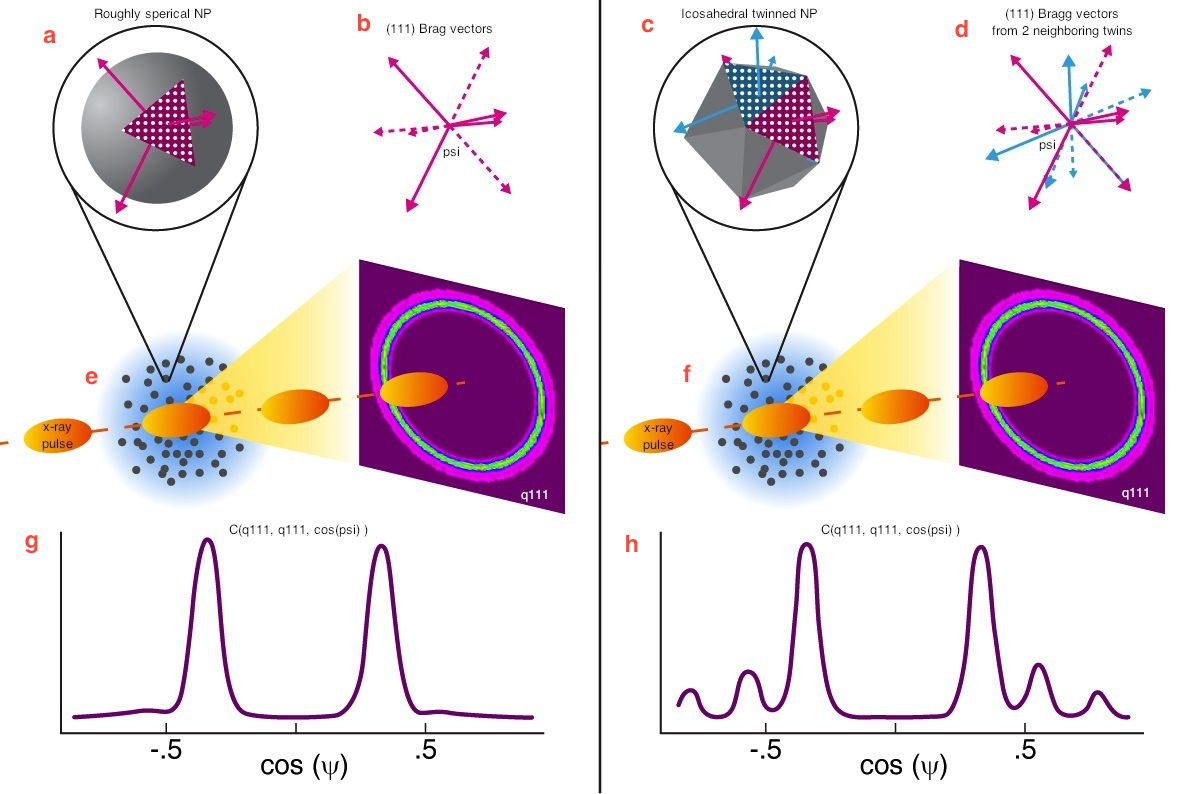
\includegraphics[width=\textwidth,height=\textheight,keepaspectratio]{./8871A01_v04_update.png}
\end{center}
\caption{Identifying twinned particles VS roughly spherical particles using CXS. \textbf{a)} A spherical face-centered-cubic NP. It is a lattice with a spherical boundary. Highlighted in pink is a tetrahedral region, whose faces are (111) planes. \textbf{b)} Bragg vectors arising from the (111) planes in the spherical NP. There are 4 (111) directions giving rise to 4 Bragg vectors. (the $180^o$ symmetric planes are shown in dashed lines). c) an icosahedral twinned particles. Highlighted are two nearest-neighbor tetrahedral regions, each akin to the one in \textbf{a)}. \textbf{d)} The Bragg vectors arising from these two neighboring twins shown in \textbf{c)}. There are more directions for photons to go, leading to additional correlation angles $\cos(\psi)$. There are correlations between next-nearest neighbor twins, but these fall off rapidly in magnitude, as there are more nearest neighbor twins. \textbf{e),f)} Powder x-ray diffraction measurements of spherical and icosahedral twinned NPs, respectively. The powder scattering signals are indistinguishable.  \textbf{g), h)} Simulations of $C(q_{111},q_{111},\cos(\psi) )$ for spherical and icosahedral twinned NPs. Bulk FCC will only produce peaks at $\pm (1/3)$ whereas nearest-neighbor twins produce peaks at $\pm (1/3), \pm (5/9), \pm (7/9)$. The height of the peaks are related to the different combinations of Bragg vectors. The two signals are clearly distinguishable. Artwork courtesy of Gregory M.~Stewart (SLAC).}
\label{fig:contrast}
\end{figure}

\begin{figure}[h]
\begin{center}
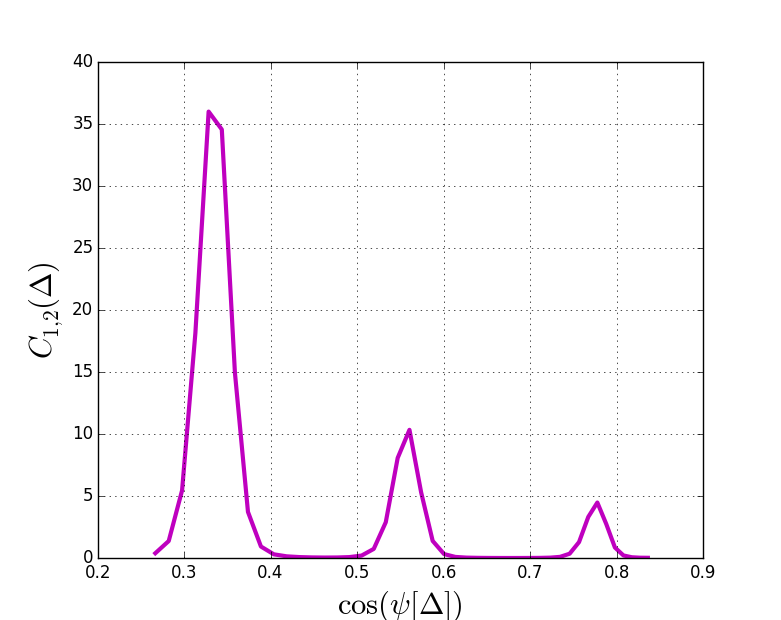
\includegraphics[width=\textwidth,height=\textheight,keepaspectratio]{./cxs_peak.png}
\end{center}
\caption{An atomic CXS simulation of (\ref{corr}) for gold NNT particles that is normalized in order to show how the peak heights agree with the predictions (\ref{psisetab}).}
\label{fig:peak}
\end{figure}




\begin{figure}[h]
\begin{center}
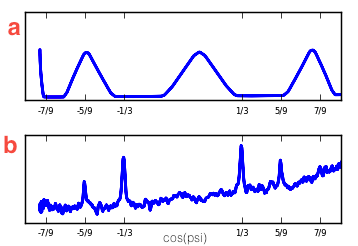
\includegraphics[width=\textwidth,height=\textheight,keepaspectratio]{./raw_dif.png}
\end{center}
\caption{\textbf{a)} Computation of $C_I(\Delta)$ for 174k exposures of gold NP solution. Shows the strong artificial correlation signal associated with experimental noise terms. b) Computation of $\widetilde C_I(\Delta)$ for 87k pairs of exposures. Without further processing, the CXS signal arising from the gold NPs in solution is clear, and clearly shows that the gold NPs are twinned.}
\label{fig:raw_dif}
\end{figure}


\begin{comment}
%We model the median-normalized intensity in a pixel at $q_{111}, \phi$ of a single exposure as

%\be
%I_s^ \phi  = \frac{ k_s^\phi \,\left( j_s^\phi  + \,n_s^\phi  \right ) }{ M_s} 
%\ee

%where $M_s$ is the median pixel value on the ring,  $j_s^\phi$ is random scattered photons coming from the background (e.g. water, buffer), and $k_s^\phi$ models the non-uniformity on the detector, due to effects such as shadows and polarization. We work with normalized intensities in order to account for fluctuation in sample volume due to small instabilities in the injector system which causes more or less photons to scatter. The $k_s^\phi$ modulations make it very difficult to extract e.g. the CXS signal (\ref{autocorr}). If one were to calculate the raw correlation

%one would notice there is very strong artificial signal associated with the correlations between the $j_s^\phi$ and $k_s^\phi$ terms. In fact, these terms make it nearly impossible to determine the signal (\ref{autocorr}); the background terms are dominant (Figure 2). Previously we reported on a binary filter method used to extract the CXS signal, however information on CXS magnitude was lost [15]. We now discuss in detail the difference correlation method for removing artificial correlations, first discussed in [14]. In general, $k_s^\phi$ is slowly varying across exposures, compared to the time between consecutive exposures. Therefore we may record the difference between two pixel intensities as

%\beq
%I_s^\phi - I_{s'}^\phi &=& k^\phi\left( \frac{j_s^\phi}{M_s} - \frac{j_{s'}^\phi}{M_{s'}}  + \frac{n_s^\phi}{M_s} - %\frac{n_{s'}^\phi}{M_{s'}} \right) \\
%&\approx& k^\phi \left( \frac{n_s^\phi}{M_s} - \frac{n_{s'}^\phi}{M_s'} \right ) \\
%&\equiv& I_{s,s'}^\phi
%\eeq



%where we assume background fluctuations between exposures ($j_s^\phi - j_{s’}^\phi$) are much less than those of the NPs. This is a fair approximation for NPs, whose scattering cross sections are typical higher than those of the solvent. Consider a variant of (\ref{rawCorr})

%\beq \label{cdif}
%\tilde{C}(\Delta) &=& \sum _s^{N_s/2} \sum_{\phi=0}^{\phi=2\pi} I_{2s, 2s+1}^\phi\,\, I_{2s,2s+1}^{\phi + \Delta} \\
%&=& \sum_{\phi=0}^{\phi=2\pi}  \tilde{C}\,^\phi( \Delta)
%\eeq

%where

\beq
\tilde{C}\,^\phi(\Delta) &=& k^\phi k^{\phi+\Delta} \sum_s^{N_s/2} \left( n_{2s}^\phi n_{2s}^{\phi+\Delta} \,+\,   n_{2s+1}^\phi n_{2s+1}^{\phi+\Delta} \,-\,  n_{2s}^\phi n_{2s+1}^{\phi+\Delta} \,-\,  n_{2s+1}^\phi\,n_{2s}^{\phi+\Delta} \right)\\
&=& k^\phi k^{\phi+\Delta }\left(  C\,^\phi(\Delta) - \sum_s^{N_s/2} \left ( n_{2s}^\phi n_{2s+1}^{\phi+\Delta} \,+\, n_{2s+1}^\phi\,n_{2s}^{\phi+\Delta}  \right) \right ) 
\eeq

Typically, $k_s^\phi$ will indeed vary throughout the course of an experiment. In this case, we cluster the exposures for which $k^\phi$ is roughly constant, compute $\tilde{C}\,^\phi(\Delta)$ for each cluster, and average the results. Terms of the form $n_s\, n_{s'}$ are statistically independent; photons scattering in shot $s$ are uncorrelated with photons scattering in shot $s'$. Therefore,

\be
\sum_s ^{N_s / 2} \left ( n_{2s}^\phi n_{2s+1}^{\phi+\Delta} \,+\,  n_{2s+1}^\phi\,n_{2s}^{\phi+\Delta} \right) \rightarrow \bar{n}^2
\ee

where $\bar{n}$ represents the average number of photons scattered by NPs measured in the pixel at $q$ and is isotropic with respect to the azimuthal. With this we have

\beq
\tilde{C}(\Delta) &=& \sum_{\phi=0}^{\phi=2\pi}  \tilde{C}\,^\phi(\Delta) \\
&=& \sum_{\phi=0}^{\phi=2\pi}  k^\phi k^{\phi+\Delta}  \left( C\,^\phi(\Delta) - \bar{n}^2    \right ) \\
\eeq

Substituting (\ref{cphi2}) into the above yields

\beq
\tilde{C}(\Delta) &=& \sum_{\phi=0}^{\phi=2\pi}  k^\phi k^{\phi+\Delta} \left( \bar{u}\,^2 + 2\,\bar{u}\bar{c} + \sum_s^{N_s}c_s^\phi c_s^{\phi + \Delta}  - \bar{n}^2  \right ) \\
&=&  \sum_{\phi=0}^{\phi=2\pi}  k^\phi k^{\phi+\Delta} \left( \bar{u}\,^2 + 2\,\bar{u}\bar{c} + \sum_s^{N_s}c_s^\phi c_s^{\phi + \Delta} - ( \bar{u} + \bar{c}  )^2 \right ) \\
&=& \sum_{\phi=0}^{\phi=2\pi}  k^\phi k^{\phi+\Delta} \left( \sum_s^{N_s}  c_s^\phi c_s^{\phi+\Delta} - \bar{c}^2 \right )
\eeq

Computation of (\ref{cdif}) for 87,000 exposures of gold NPs from SACLA is shown in Figure 2. While we only have empirical evidence to support the power of (\ref{cdif}), the results are striking.

\section{Discussion}
An elementary gold NP model consists of an (FCC) lattice with a spherical boundary (Figure 1a, 1g). Let $\{\bm q_{111}\}$ be the set of all $\{111\}$ Bragg vectors. By considering all pairs of vectors $\bm q_1, \bm q_2 \in \{\bm q_{111}\}$ one can show that $\cos (\psi)$ can only take on values $\pm (1/3)$. 


These values are precisely the peak locations shown in Figure 1h and Figure 2b. Previously, when we reported on CXS of silver NPs, we only observed peaks at $\cos(\psi) = \pm (1/3)$, however their we made use of a non-linear binary filter which reduced the information content. Further, the amount of data (15k exposures) was limited due to the typically long exposure times at synchrotrons compared to those at SACLA. Prior to analyzing the SACLA dataset, we have computed (\ref{cdif}) for the SSRL dataset, and first took note of what appeared to be additional CXS peaks (Figure 3), which were not predicted by the elementary NP model (Figure 1a). This was initially puzzling, but after comparing with the SACLA gold NP dataset (Figure 3), we realized these correlations were in fact real, and were representing a more general property of small FCC NPs.

In order to see the power of the difference correlation, one must split $n$ as a sum of correlated photons $c$ and uncorrelated photons $u$. 

\beq
C_\phi &=& \sum _s^{N_s} (c_s + u_s ) ( c_s^\Delta + u_s^\Delta) \\
&=&\sum _s^{N_s} \left( c_s c_s^\Delta + c_s u_s^\Delta + u_s c_s^\Delta + u_s u_s^\Delta \right ) \\
&=&\sum _s^{N_s} \left( c_s c_s^\Delta + c_s u_s^\Delta \right )+ \bar{u}\bar {n}^\Delta
\eeq

\section{Supplemental}
Correlated x-ray scattering (CXS) is an emerging technique that aims to extract structural information from ensmble  scattering measurements. We define the sample ensemble as a set of identical, non-interacting objects $\{m\}$, each with an independent orientation $\omega$ relative to the x-ray beam axis, governed by the object's diffusion constant. We consider each object $m$ as a collection of $N_a$ atoms each with position vector 
\be
\bm r^m_j (t) = \bm R^m_\omega (t)\cdot \bm r_j + \bm T^m(t) \qquad 1 \le j \le N_a
\ee 
where $\bm R^m_\omega(t)$ is a rotation operator, $\bm T^m (t)$ is a translation operator representing the center of mass position of $m$ at time $t$, and $\bm r_j$ is the position of the $j^{th}$ atom at an arbitrarily defined initial orientation. If we were to freeze the solution at an instant in time and expose it to x-ray photons of wavelength $\lambda$, then we could measure the scattering function
\be
S(\bm q, t) = \left | \sum_m \sum_{j}^{N_a} f_j(q) \,e ^ { -i \,\bm q \cdot \bm  r^m _j (t)  } \right |^2
\ee
Here $f_j( q  )$ is the atomic form factor of the $j^{th}$ atom$, \bm q$ represents a position in reciprocal space (e.g. of a pixel) at scattering angle  
\be \label{angle}
\sin(\theta) = \frac{ \lambda }{ 4 \pi}\,q
\ee
and the outer sum is over all exposed $m$. In general, $S(\bm q, t)$ may be written as
\be \label{ sums }
S( \bm q, t) = \sum_m \left | A^m_\omega (\bm q ) \right|^2 + \sum _{ m \neq m' } A^m_\omega (\bm q) \left (A^{m'}_\omega (\bm q) \right )^*
\ee
where 
\be
A^m_\omega (\bm q) = \sum_{j}^{N_a} f_j(q) e^{ -i \,\bm q \cdot \bm  r^m_j (t)  }
\ee

The strength of the interference term on the RHS of (\ref{ sums }) depends on both the concentration of the sample, and the magnitude of the scattering angle (\ref{angle}). In what follows we will work at relatively high scattering angles, hence we can safely neglect this limit such that we have

\beq \label{ scatter}
S( \bm q, t) &=& \sum_m \left | A^m_\omega (\bm q) \right|^2 \\
&=& \sum_m \left | \sum_{j}^{N_a} f_j(q)\, e^ { -i \,\bm q \cdot \bm  r^m _j (t)} \right | ^2   \\
&=& \sum_m \left | \sum_{j}^{N_a} f_j(q)\, e^ { -i \,\bm q \cdot \left (\bm {R}^m_\omega \left(t\right)\cdot \bm r_j \,+\, \bm {T}^m\left(t\right) \right)} \right | ^2 \\
&=& \sum_m \left | \sum_{j}^{N_a} f_j(q)\, e^ { -i \,\bm q \cdot \bm {R}^m_\omega (t)\cdot \bm r_j }  \right | ^2 
\eeq

After exposing the solution for a finite time interval $\tau$, a pixel at $\bm q$ will record 

\be
n_s( \bm q ) \propto \int_{\tau} S( \bm q, t ) d\tau
\ee

photons, where $s$ is used to denote a unique exposure, referred to as a ``shot". 
%For sufficiently long $\tau$, the number of photons scattered from objects in each orientation $\omega$ becomes a constant and $n_s(\bm q)$ approaches a well defined average value
%\be
%\int_{\tau} dt \sum_m  \xrightarrow{\tau \rightarrow \infty} \frac{N_m}{8\pi^2}\int d\omega
%\ee
%and we have
for each shot it is convenient to define an angular average over the azimuthal angle $\phi$ as
\be 
\bar{n}_s(q)=\sum_{\phi} n_s( \bm q,\phi ) 
\ee
However, provided $\tau$ is much shorter than the characteristic diffusion time, one can measure a finite  deviationof the scattering
\be \label{delta_s}
\delta n_s(\bm q) = n_s (\bm q) - \bar {n}_s (q )
\ee

By recording many exposures, each representing a different state of the solution frozen in time, one can construct a correlation function
\be \label{delta_cor}
C( \bm q_1, \bm q_2 ) = \sum_s^{N_s} \delta n_s( \bm q_1 )\, \delta n_s( \bm q_2 ) = \sum_s^{N_s} \left \{n_s( \bm q_1) n_s (\bm q_2 )  - \bar n_s( q_1) \bar n_s(q_2)\right \}
\ee
which contains detailed information beyond that contained in the isotropic $\bar n( q)$. To understand the information content stored in (\ref{delta_cor}), one must again consider the solution frozen in time (if $\tau$ is sufficiently small then this is a valid approximation). In the limit that the flux is so weak that  the probability for one object to scatter two photons tends to zero, then only single scattering occurs into random directions and $C \rightarrow 0$. 
\end{comment}


\section{References}

1. Kam Z. 1977 Determination of macromolecular structure in solution by spatial correlation of scattering fluctuations. Macromolecules 10:927–934. (doi:10.1021/ma60059a009)

2. Narayanan R and El-Sayed MA ,2005, Catalysis with Transition Metal Nanoparticles in Colloidal Solution: Nanoparticle Shape Dependence and Stability J. Phys. Chem. B, 109, 12663-12676

3. Radha Narayanan and Mostafa A. El-Sayed, Shape-Dependent Catalytic Activity of Platinum Nanoparticles in Colloidal Solution, Nano Lett., Vol. 4, No. 7, 2004

4. Marks, L. D. Modified Wulff Constructions for Twinned Particles. J. Cryst. Growth 1983, 61, 556‚àí566.

5. Ringe E dx.doi.org/10.1021/jp401566m | J. Phys. Chem. C 2013, 117, 15859‚àí15870

6. Stepwise Evolution of Spherical Seeds into 20-Fold Twinned Icosahedra Mark R. Langille et al. Science 337, 954 (2012); DOI: 10.1126/science.1225653

7. C.Y. YANG Journal of Crystal Growth 47 (1979) 274—282

8. C.Y.YANG, M.J.YACAMAN K.HEINEMANN Journal of Crystal Growth 47 (1979) 283—290

9. Marks, L. D.; Smith, D. J. High-Resolution Studies of Small Particles of Gold and Silver 0.1. Multiply-Twinned Particles. J. Cryst. Growth 1981, 54, 425‚àí432.

10. Chien-Chun Chen et al Nature 496, 74–77 (04 April 2013) doi:10.1038/nature12009

11. Friedel G (1913) Sur les symetries cristallines que peut reveler la diffraction des rayons Rontgen. Comptes Rendus hebdo-madaires de l’Academie des Sciences 157:1533–1536

12. Kirian RA,Schmidt KE,Wang X,Doak RB,Spence JCH. 2011 Signal, noise, and resolution in correlated fluctuations from snapshot small-angle X-ray scattering . Phys. Rev. E 84, 011921. (doi:10.1103/PhysRevE.84.011921)

13. Neutze R,Wouts R,van der Spoel D,Weckert E,Hajdu J. 2000 Potential for biomolecular imaging with femtosecond X-ray pulses. Nature 406, 752–757. (doi:10.1038/35021099)

14. Kam Z,Koch MH,Bordas J. 1981 Fluctuation X-ray scattering from biological particles in frozen solution by using synchrotron radiation. Proc. Natl Acad. Sci. USA 78, 3559–3562. (doi:10.1073/pnas.78.6.3559)

15. Mendez et al, 2014,  Observation of correlated X-ray scattering at atomic resolution, Phil Trans R Soc B 369: 20130315


\end{document}






